\documentclass[tikz,border=1mm,10pt,dvipsnames]{standalone}

\usetikzlibrary{shapes.misc}
\tikzset{cross/.style={cross out, draw=black, minimum size=2*(#1-\pgflinewidth), inner sep=0pt, outer sep=0pt},
%default radius will be 1pt.
cross/.default={1pt}}

\begin{document}
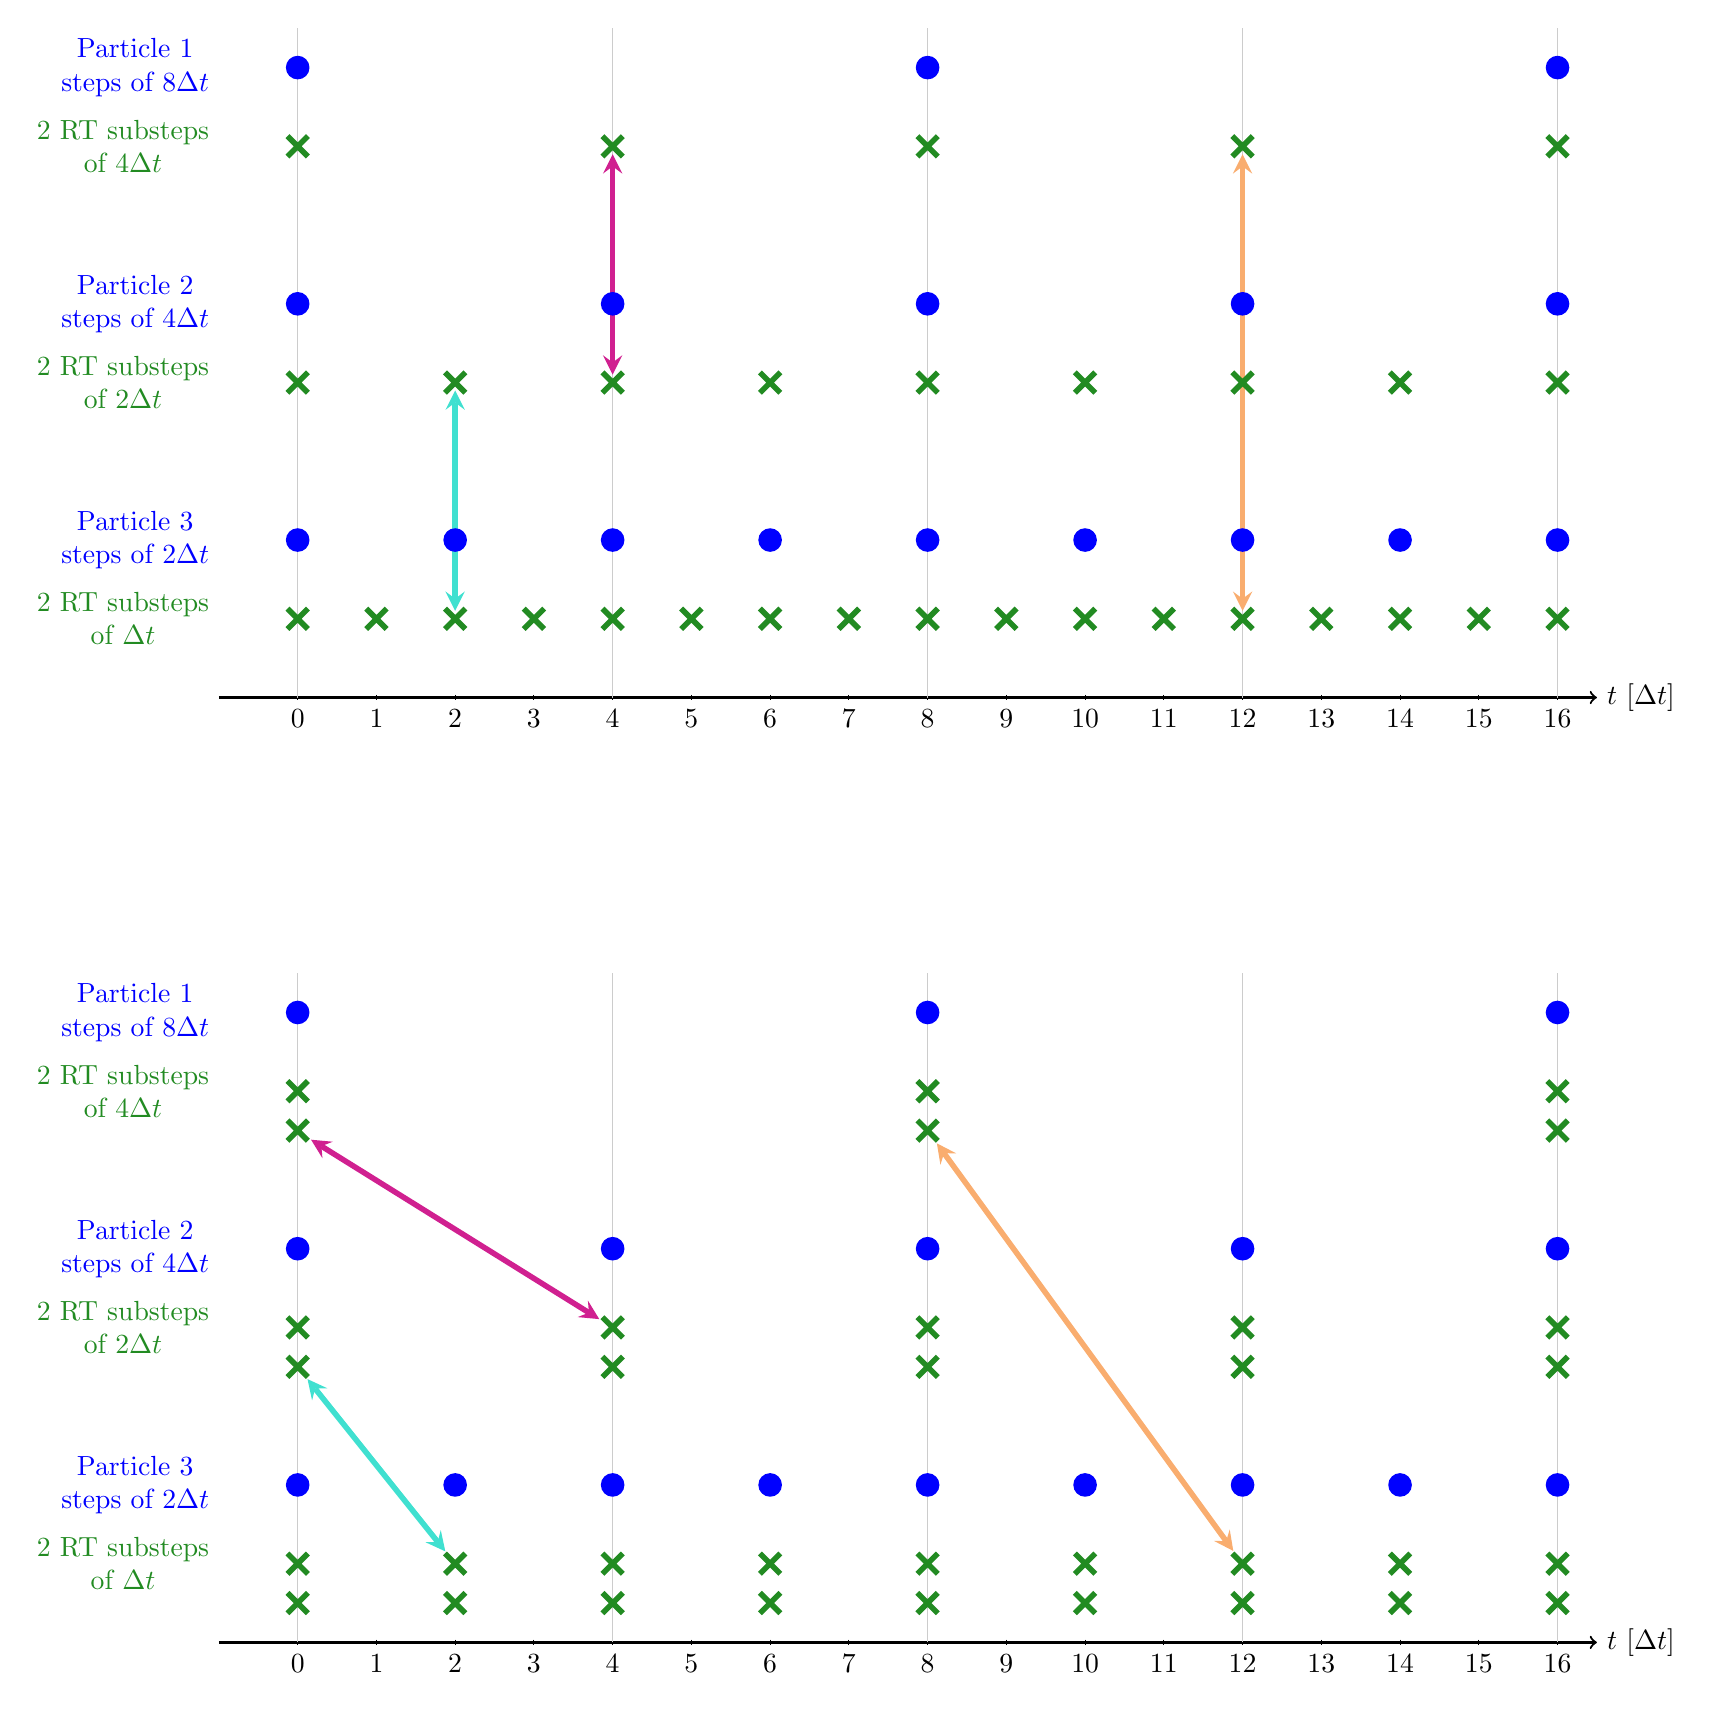
\begin{tikzpicture}%[xscale=1,yscale=1,samples=400, transform shape,every node/.style={scale=0.7}]


	\pgfdeclarelayer{bg}    % declare background layer
	\pgfsetlayers{bg,main}  % set the order of the layers (main is the standard layer)

	\def\hydroColor{blue};
	\def\rtColor{ForestGreen};

	\def\Xzero{-1cm};
	\def\Xmax{16.5cm};
	\def\Yzero{0cm};
	\def\Ymax{8.5cm};
	\def\partoneY{8cm};
	\def\parttwoY{5cm};
	\def\partthreeY{2cm};

	\def\radius{0.15cm};
	\def\rtOffset{1cm};
	\def\rtCross{node[cross=.2cm,rotate=0, \rtColor, line width=2pt]{}};

\begin{pgfonlayer}{bg}    % select the background layer
	% X Axis
	\draw[thick, ->] (\Xzero,\Yzero) -- (\Xmax,\Yzero) node[anchor=west] {$t$ [$\Delta t]$};
	\foreach \x in {0,1,2,3,4,5,6,7,8,9,10,11,12,13,14,15,16}
		\draw (\x cm,1pt) -- (\x cm,-1pt) node[anchor=north] {$\x$};

	% Y Axis
%	\draw[thick] (-1,0) -- (-1,8.5); %node[anchor=south east] {y axis};
	% Axes ticks
%	\foreach \y in {0,1,2,3,4,5,6,7,8}
%		\draw (\Xzero-1pt,\y cm) -- (\Xzero-1pt,\y cm) node[anchor=east] {$\y$};

	% Grey background lines
	\foreach \x in {0, 4, 8, 12, 16}
		\draw [color=gray!40] (\x,\Yzero) -- (\x,\Ymax);
\end{pgfonlayer}

	% Particle labels
	\draw node[anchor=east, align=center, \hydroColor] at (\Xzero, \partoneY) {Particle 1\\ steps of $8 \Delta t$};

	\draw node[anchor=east, align=center, \hydroColor] at (\Xzero, \parttwoY) {Particle 2\\ steps of $4 \Delta t$};

	\draw node[anchor=east, align=center, \hydroColor] at (\Xzero, \partthreeY) {Particle 3\\ steps of $2 \Delta t$};


	% RT labels
	\draw node[anchor=east, align=center, \rtColor] at (\Xzero, \partoneY-\rtOffset) {2 RT substeps\\ of $4 \Delta t$};

	\draw node[anchor=east, align=center, \rtColor] at (\Xzero, \parttwoY-\rtOffset) {2 RT substeps\\ of $2 \Delta t$};

	\draw node[anchor=east, align=center, \rtColor] at (\Xzero, \partthreeY-\rtOffset) {2 RT substeps\\ of $\Delta t$};




	% Particle 1 Hydro Activity
	\foreach \px in {0, 8, 16}
		\fill[color=\hydroColor] (\px,\partoneY) circle (\radius);


	% Particle 2 Hydro Activity
	\foreach \px in {0, 4, 8, 12, 16}
		\fill[color=\hydroColor] (\px,\parttwoY) circle (\radius);


	% Particle 3 Hydro Activity
	\foreach \px in {0, 2, 4, 6, 8, 10, 12, 14, 16}
		\fill[color=\hydroColor] (\px,\partthreeY) circle (\radius);


	% Particle 1 RT Activity
	\foreach \px in {0, 4, 8, 12, 16}
		\draw (\px,\partoneY-\rtOffset) \rtCross;

	% Particle 2 RT Activity
	\foreach \px in {0, 2, 4, 6, 8, 10, 12, 14, 16}
		\draw (\px,\parttwoY-\rtOffset) \rtCross;

	% Particle 3 RT Activity
	\foreach \px in {0, 1, 2, 3, 4, 5, 6, 7, 8, 9, 10, 11, 12, 13, 14, 15, 16}
		\draw (\px,\partthreeY-\rtOffset) \rtCross;

  \begin{pgfonlayer}{bg}    % select the background layer
		% Arrow 1
		\draw [color=Turquoise, line width = 2pt, stealth-stealth, shorten >=0.1cm,shorten <=0.1cm] (2, \parttwoY - \rtOffset) -- (2, \partthreeY - \rtOffset);

		% Arrow 2
		\draw [color=VioletRed, line width = 2pt, stealth-stealth, shorten >=0.1cm,shorten <=0.1cm] (4, \partoneY - \rtOffset) -- (4, \parttwoY - \rtOffset);

		% Arrow 3
		\draw [color=Apricot, line width = 2pt, stealth-stealth, shorten >=0.1cm,shorten <=0.1cm] (12, \partoneY - \rtOffset) -- (12, \partthreeY - \rtOffset);
	\end{pgfonlayer}


%-------------------------------------------------------------------------------
% Lower Plot
%-------------------------------------------------------------------------------

	\def\plotoffset{-12cm};
	\def\Xzero{-1cm};
	\def\Xmax{16.5cm};
	\def\Yzero{0cm + \plotoffset};
	\def\Ymax{8.5cm + \plotoffset};
	\def\partoneY{8cm + \plotoffset};
	\def\parttwoY{5cm + \plotoffset};
	\def\partthreeY{2cm + \plotoffset};

\begin{pgfonlayer}{bg}    % select the background layer
	% X Axis
	\draw[thick, ->] (\Xzero,\Yzero) -- (\Xmax,\Yzero) node[anchor=west] {$t$ [$\Delta t]$};
	\foreach \x in {0,1,2,3,4,5,6,7,8,9,10,11,12,13,14,15,16}
		\draw (\x cm,1pt+\plotoffset) -- (\x cm,-1pt+\plotoffset) node[anchor=north] {$\x$};

	% Y Axis
%	\draw[thick] (-1,0) -- (-1,8.5); %node[anchor=south east] {y axis};
	% Axes ticks
%	\foreach \y in {0,1,2,3,4,5,6,7,8}
%		\draw (\Xzero-1pt,\y cm) -- (\Xzero-1pt,\y cm) node[anchor=east] {$\y$};

	% Grey background lines
	\foreach \x in {0, 4, 8, 12, 16}
		\draw [color=gray!40] (\x,\Yzero) -- (\x,\Ymax);
\end{pgfonlayer}

	% Particle labels
	\draw node[anchor=east, align=center, \hydroColor] at (\Xzero, \partoneY) {Particle 1\\ steps of $8 \Delta t$};

	\draw node[anchor=east, align=center, \hydroColor] at (\Xzero, \parttwoY) {Particle 2\\ steps of $4 \Delta t$};

	\draw node[anchor=east, align=center, \hydroColor] at (\Xzero, \partthreeY) {Particle 3\\ steps of $2 \Delta t$};


	% RT labels
	\draw node[anchor=east, align=center, \rtColor] at (\Xzero, \partoneY-\rtOffset) {2 RT substeps\\ of $4 \Delta t$};

	\draw node[anchor=east, align=center, \rtColor] at (\Xzero, \parttwoY-\rtOffset) {2 RT substeps\\ of $2 \Delta t$};

	\draw node[anchor=east, align=center, \rtColor] at (\Xzero, \partthreeY-\rtOffset) {2 RT substeps\\ of $\Delta t$};



	% Particle 1 Hydro Activity
	\foreach \px in {0, 8, 16}
		\fill[color=\hydroColor] (\px,\partoneY) circle (\radius);


	% Particle 2 Hydro Activity
	\foreach \px in {0, 4, 8, 12, 16}
		\fill[color=\hydroColor] (\px,\parttwoY) circle (\radius);


	% Particle 3 Hydro Activity
	\foreach \px in {0, 2, 4, 6, 8, 10, 12, 14, 16}
		\fill[color=\hydroColor] (\px,\partthreeY) circle (\radius);


	% Particle 1 RT Activity
	\foreach \px in {0, 8, 16}
		\draw (\px,\partoneY-\rtOffset) \rtCross;
	\foreach \px in {0, 8, 16}
		\draw (\px,\partoneY-1.5*\rtOffset) \rtCross;

	% Particle 2 RT Activity

	\foreach \px in {0, 4, 8, 12, 16}
		\draw (\px,\parttwoY-\rtOffset) \rtCross;
	\foreach \px in {0, 4, 8, 12, 16}
		\draw (\px,\parttwoY-1.5*\rtOffset) \rtCross;


	% Particle 3 RT Activity
	\foreach \px in {0, 2, 4, 6, 8, 10, 12, 14, 16}
		\draw (\px,\partthreeY-\rtOffset) \rtCross;
	\foreach \px in {0, 2, 4, 6, 8, 10, 12, 14, 16}
		\draw (\px,\partthreeY-1.5*\rtOffset) \rtCross;


  \begin{pgfonlayer}{bg}    % select the background layer
		% Arrow 1
		\draw [color=Turquoise, line width = 2pt, stealth-stealth, shorten >=0.2cm,shorten <=0.2cm] (0, \parttwoY - 1.5 * \rtOffset) -- (2, \partthreeY - \rtOffset);

		% Arrow 2
		\draw [color=VioletRed, line width = 2pt, stealth-stealth, shorten >=0.2cm,shorten <=0.2cm] (0, \partoneY - 1.5 \rtOffset) -- (4, \parttwoY - \rtOffset);

		% Arrow 3
		\draw [color=Apricot, line width = 2pt, stealth-stealth, shorten >=0.2cm,shorten <=0.2cm] (8, \partoneY - 1.5 * \rtOffset) -- (12, \partthreeY - \rtOffset);
	\end{pgfonlayer}


\end{tikzpicture}
\end{document}